\section{Toolchain}

MARK II is not only SoC, there is also several tools that will help you to
write software for MARK II. They are writen in Python and are placed in tools
directory. Tools are primary intended for using under linux with python 2.7.
Typical workflow is on image \ref{fig:toolchain_workflow}, and tools consist
from following parts.

\begin{itemize}
    \item \textbf{Assembler} - translate programs from symbolic language into machine code
    \item \textbf{Linker} - link multiple object files into loader module
    \item \textbf{Emulator} - emulate part of the SoC
    \item \textbf{Disassembler} - disassemble programs from machine code
    \item \textbf{ldm2mif} - script that convert loader module into mif and also can perform relocation
    \item \textbf{Loader} - perform relocation and load program into memory with serial bootloader
\end{itemize}

\begin{figure}[]
    \centering
    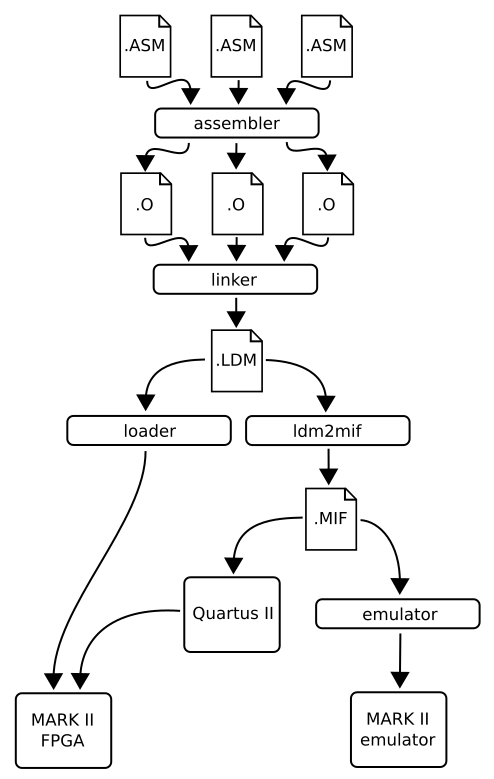
\includegraphics[width=.7\textwidth]{img/toolworkflow.png}
    \caption{MARK-II Toolchain - typical workflow}
    \label{fig:toolchain_workflow}
\end{figure}
